\section{Package Model}\begin{figure}[h!]
\begin{center}
	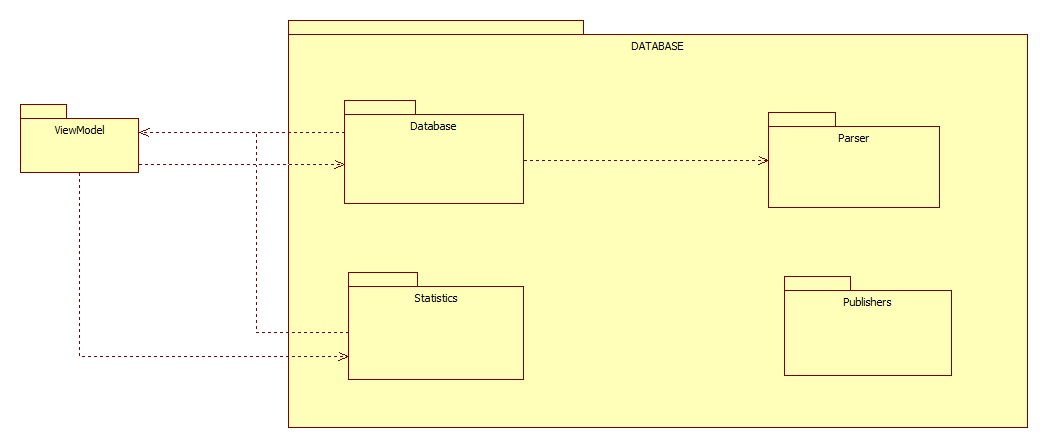
\includegraphics[scale=0.4]{../images/ModelPackage.jpg}
\end{center}
\end{figure}
\subsection{Model::Database}
\subsubsection{Model::Database::QuizManager}
\begin{itemize}
\item\textbf{Funzione del componente:} la classe permettera' l'inserimento, la lettura e la rimozione di questionari all'interno della collezione
\item\textbf{Relazioni d'uso con altre componenti:} Model::Publishers::QuizPublisher; Model::Statistics::Statistics\\
\item\textbf{Metodi}:
\begin{itemize}
	\item\code{+ quizzes.insert()} : Metodo per aggiungere un nuovo quiz al database\\
	\textbf{Parametri}:
	\begin{itemize}
		\item\code{owner: string}\\
		\item\code{title: string}\\
		\item\code{time: int}\\
		\item\code{questions: array}\\
		\item\code{categories: array}\\
		\item\code{createdAt: date}\\
		\textbf{Precondizioni}: Vengono richiesti i dati necessari per la creazione e il salvataggio di un quiz\\
		\textbf{Postcondizioni}: Il quiz e' stato salvato correttamente nel database e crea una entry corrispondente nella collezione delle statistiche\\
	\end{itemize}
	\item\code{+ quizzes.update()} :  Metodo per modificare un quiz nel database\\
	\textbf{Parametri}:
	\begin{itemize}
		\item\code{quizID: string}\\
		\item\code{title: string}\\
		\item\code{time: int}\\
		\item\code{questions: array}\\
		\item\code{categories: array}\\
		\textbf{Precondizioni}: Vengono richiesti i dati necessari per la modifica di un quiz\\
		\textbf{Postcondizioni}: Il quiz e' stato modificato nel database\\
	\end{itemize}
	\item\code{+ quizzes.remove()} : Metodo per rimuovere un quiz dal database\\
	\textbf{Parametri}:
	\begin{itemize}
		\item\code{quizID: string}\\
		\textbf{Precondizioni}: Vengono richiesti i dati necessari per la rimozione di un quiz\\
		\textbf{Postcondizioni}: Il quiz e' stato rimosso dal database e le statistiche ad esso associate vengono anch'esse rimosse\\
	\end{itemize}
\end{itemize}
\end{itemize}

\subsubsection{Model::Database::QuestionManager}
\begin{itemize}
\item\textbf{Funzione del componente:} la classe permettera' l'inserimento, la modifica e la rimozione di singoli quesiti all'interno della collezione
\item\textbf{Relazioni d'uso con altre componenti:} Model::Publishers::QuizPublisher; Model::Statistics::Statistics; Model::Interpreter::Interpreter\\
\item\textbf{Metodi}:
	\begin{itemize}
		\item\code{+ questions.insert()} : Metodo per aggiungere un nuovo quesito al database\\
		\textbf{Parametri}:
			\begin{itemize}
				\item\code{QMLtext: string}\\
				\item\code{category: string}\\
				\textbf{Precondizioni}: Vengono forniti i dati necessari per la creazione e il salvataggio di un nuovo quesito (il testo QML e la categoria vengono immessi dall'utente mentre data e utente corrente sono informazioni già presenti il sistema al momento della richiesta)\\
				\textbf{Postcondizioni}: Il quesito e' stato salvato correttamente nel database se viene rispettata la sintassi QML, altrimenti viene restituito un messaggio d'errore\\
			\end{itemize}
		\item\code{+ questions.update()} : Metodo per modificare un quesito nel database\\
		\textbf{Parametri}:
			\begin{itemize}
				\item\code{questionID: string}\\
				\item\code{QMLtext: string}\\
				\item\code{category: string}\\
				\textbf{Precondizioni}: Vengono forniti i dati necessari per la modifica di un intero quesito o di sue parti (es. solo alcune parti del testo o cambio di categoria)\\
				\textbf{Postcondizioni}: Il quesito e' stato modificato nel database se viene rispettata la sintassi QML, altrimenti viene restituito un messaggio d'errore\\
			\end{itemize}
		\item\code{+ questions.remove()} : Metodo per rimuovere un quesito dal database\\
		\textbf{Parametri}:
			\begin{itemize}
				\item\code{questionID: string}\\
				\textbf{Precondizioni}: L'utente richiede l'eliminazione di un quesito\\
				\textbf{Postcondizioni}: Il quesito e' stato rimosso dal database\\
			\end{itemize}
	\end{itemize}
\end{itemize}

\subsubsection{Model::Database::Search}
\begin{itemize}
\item\textbf{Funzione del componente:} la classe permettera' la ricerca di sottostringhe in singoli quesiti o in diversi questionari 
\item\textbf{Relazioni d'uso con altre componenti:} Model::Publishers::QuizPublisher; MOdel::Publishers::QuestionPublisher\\
\item\textbf{Metodi}:
\begin{itemize}
	\item\code{+ question.search()} : Metodo per ricercare una stringa all'interno di tutte le domande\\
	\textbf{Parametri}:
	\begin{itemize}
		\item\code{string: string}\\
		\textbf{Precondizioni}: Viene fornito il parametro che si vuole ricercare\\
		\textbf{Postcondizioni}: Vengono restituite tutte le domande che contengono il parametro\\
	\end{itemize}
	\item\code{+ quizzes.search()} :  Metodo per ricercare una stringa all'interno di tutti i questionari\\
	\textbf{Parametri}:
	\begin{itemize}
		\item\code{string: string}\\
		\textbf{Precondizioni}: Viene fornito il parametro che si vuole ricercare\\
		\textbf{Postcondizioni}: Vengono restituite tutti i questionari che rispecchiano i criteri di ricerca\\
	\end{itemize}
\end{itemize}
\end{itemize}

\subsection{Model::Parser}
\subsubsection{Model::Parser::Parser}
\begin{itemize}
\item\textbf{Funzione del componente:} controlla che il testo fornito risulti corretto secondo la sintassi QML
\item\textbf{Relazioni d'uso con altre componenti:} QuestionManager\\
\item\textbf{Metodi}:
	\begin{itemize}
		\item\code{+ check()} : Metodo per controllare che un nuovo quesito rispetti la sintassi QML prima di essere aggiunto al database\\
		\textbf{Parametri}:
			\begin{itemize}
				\item\code{testo\_da\_controllare: string}\\
				\textbf{Precondizioni}: Viene richiesta una string che contiene la domanda\\
				\textbf{Postcondizioni}: Viene restituito un messaggio contenente il risultato dell'operazione di controllo sintattico\\
			\end{itemize}
	\end{itemize}
\end{itemize}

\subsection{Model::Statistics}
\subsubsection{Model::Statistics::Statistics}
\begin{itemize}
\item\textbf{Funzione del componente:} questa classe fornisce funzionalita' per il raccoglimento delle statistiche sulle prestazioni degli utenti del sistema
\item\textbf{Relazioni d'uso con altre componenti:} Model::Publishers::QuizPublishers; Model::Publishers::questionPublishers\\
\item\textbf{Metodi}:
\begin{itemize}
	\item\code{+ statistics.QuizExecutionStats()} : Metodo per aggiornare le statistiche di un quesito nel database\\
	\textbf{Parametri}:
	\begin{itemize}
		\item\code{QuizObject: JSON object}\\
		\item\code{UserID: string}\\
		\textbf{Precondizioni}: L'utente ha consegnato il questionario\\
		\textbf{Postcondizioni}: Le statistiche relative ad ogni domanda contenuta nel questionario sono state aggiornate\\
	\end{itemize}
	\item\code{+ statistics.UserExecutionStats()} : Metodo per aggiornare le statistiche sulla performance di un utente registrato\\
	\textbf{Parametri}:
	\begin{itemize}
		\item\code{UserID: string}\\
		\item\code{QuestionAnswered: array/string/int}\\
		\item\code{QuestionCorrectAnswered: array/string/int}\\
		\textbf{Precondizioni}: L'utente registrato ha consegnato un questionario\\
		\textbf{Postcondizioni}: Vengono aggiornate le statistiche totali di quell'utente\\
	\end{itemize}
	\item\code{+ statistics.QuestionExecutionStats()} : Metodo per aggiornare le statistiche di un quiz nel database\\
	\textbf{Parametri}:
	\begin{itemize}
		\item\code{QuestionID: string}\\
		\item\code{Correct: bool}\\
		\textbf{Precondizioni}: L'utente ha dato una risposta alla domana\\
		\textbf{Postcondizioni}:La risposta (corretta o meno) viene integrata nelle statistiche\\
	\end{itemize}
\end{itemize}
\end{itemize}

\subsection{Model::Publishers}
\subsubsection{Model::Publishers::QuizPublisher}
\begin{itemize}
\item\textbf{Funzione del componente:} questa classe fornisce funzionalita' per rendere pubblica la collezione dei quiz all'avvio del Sistema
\item\textbf{Relazioni d'uso con altre componenti:} Nessuna \\
\item\textbf{Metodi}:
	\begin{itemize}
		\item\code{+ Meteor.publish()} : Metodo per rendere accessibili la collezione dei quiz all'avvio del Sistema\\
		\textbf{Precondizioni}: Il Sistema non ha ancora reso pubblica la collezione dei quiz\\
		\textbf{Postcondizioni}: Il Sistema ha reso pubblica la collezione dei quiz\\
	\end{itemize}
\end{itemize}

\subsubsection{Model::Publishers::QuestionPublisher}
\begin{itemize}
\item\textbf{Funzione del componente:} questa classe fornisce funzionalita' per rendere pubblica la collezione dei quesiti all'avvio del Sistema
\item\textbf{Relazioni d'uso con altre componenti:} Nessuna \\
\item\textbf{Metodi}:
	\begin{itemize}
		\item\code{+ publishQuestion()} : Metodo per rendere accessibili la collezione dei quesiti all'avvio del Sistema\\
		\textbf{Precondizioni}: Il Sistema non ha ancora reso pubblica la collezione dei quesiti\\
		\textbf{Postcondizioni}: Il Sistema ha reso pubblica la collezione dei quesiti\\
	\end{itemize}
\end{itemize}